%%+++++++++++++++++++++++++++++++++++++%%
%%         Final Version  6/14/95      %%
%%+++++++++++++++++++++++++++++++++++++%%
\documentclass[12pt]{article}
\textheight = 8.6in
\textwidth = 6.2in
\topmargin = -.5in
\oddsidemargin = 0.08in
\evensidemargin = 0.08in
%\usepackage{fancyhdr}
%\pagestyle{fancy}
%\rfoot{\thepage}
\setlength{\jot}{10.0 pt}
\setlength{\parskip}{2.5ex}
\setlength{\footskip}{65pt}

\usepackage{graphicx}
\usepackage{subfigure}
\usepackage{placeins}
\usepackage{afterpage}
\usepackage{amsmath}
\usepackage{empheq}
\usepackage[most]{tcolorbox}
\newtcbox{\mymath}[1][]{%
    nobeforeafter, math upper, tcbox raise base,
    enhanced, colframe=white!20!black ,
    colback=blue!30!red!30!white, boxrule=1pt,
    #1}
\usepackage{xcolor}
\definecolor{myblue}{RGB}{0, 0, 180}   %Numbers are integers from 0 to 255, smaller is closer to black
\definecolor{grey}{RGB}{200, 200, 200}   %Numbers are integers from 0 to 255, smaller is closer to black
\definecolor{mygreen}{RGB}{0, 100, 0}   %Numbers are integers from 0 to 255, smaller is closer to black
\definecolor{myred}{RGB}{120, 0, 0}   %Numbers are integers from 0 to 255, smaller is closer to black

\begin{document}

\begin{flushright} {\color{blue} Chapter 3, Lecture 2} \end{flushright}
\begin{flushleft}

\iffalse
%Uniqueness - probably goes elsewhere
{\color{grey} \hrulefill}\\
Found a solution?  No worries, it is the only possible solution:\\
\vspace{.1in}

The uniqueness theorem says that if you find \textbf{\textit{a}} solution to the problem, it is \textbf{\textit{the}} solution to the problem.  As stated in Griffiths;
\vspace{-.1in}
\begin{enumerate}
\item ``The solution to Laplace's equation in some volume is uniquely determined if the potential is specified on the boundary surface.''\\
\item Or - ``In a volume surrounded by conductors with charge density $\rho$, the electric field is uniquely determined if the total charge on each conductor is given.''\\
\end{enumerate}
\vspace{-.3in}
{\color{grey} \hrulefill}\\
\fi

\subsubsection*{\color{myblue} \bf Introduction to expansions of harmonic functions}

\subsubsection*{\color{mygreen} \bf General discussion}

A solution to a problem described with Laplace's equation can often be found using the method of the separation of variables.  Then, the solution is not in closed form but is a sum of harmonic functions.  These harmonic functions are members of a complete, orthogonal set of functions.  Boundary conditions are needed to determine the coefficients of each harmonic function in the series to obtain the specific solution.

You've encountered two ideas incorporated in expansions of orthogonal functions before:
\vspace{-.1in}
\begin{enumerate}
\item A function may be approximated by a sum of terms such as in a Taylor expansion.\\
\item An arbitrary vector can be represented by resolving it into components.  A useful coordinate system offers a complete basis of orthogonal unit vectors from which any arbitrary vector may be constructed.\\
\end{enumerate}

\subsubsection*{\textbf{\color{mygreen} Approximating a function with an expansion}}

The value of a (differentiable) function in the neighborhood of a specific point $x$ may be approximated as a sum of terms with the displacement from that point, $h$, in successively higher powers.  If the function is linear, then $f(x+h)=f(x) + h\frac{\partial f(x)}{\partial x}$; the first two terms accurately describe the new value of the function at $x+h$.  No matter what the curvature of the function between $x$ and $x+h$, with more terms in the expansion an accurate representation can be constructed for the value of the function at the neighboring point, $f(x+h)$.  Such an expansion (very roughly described here) is a Taylor expansion, one form is given in Eq.~\ref{eq:taylor}.

\begin{equation}
f(x+h)=\sum_{n=0}^{\infty} \frac{h^{n}}{n!}\frac{d^{n}f(x)}{dx^{n}}=f(x)+h\frac{df(x)}{dx}+\frac{h^{2}}{2}\frac{d^{2}f(x)}{dx^{2}}+\dots
\label{eq:taylor}
\end{equation}

Next up is a Taylor expansion example, for the sine function $f(t)=\sin{(t)}$, expanded around $t=0$.  
Here the expansion is around the point $t=0$, at a small displacement $t$.  The Taylor expansion in this case may be written as, 
\begin{equation}
f(t) = \sin{(0+t)} = C_{0} + C_{1}t + C_{2}t^{2} + C_{3}t^{3} + \dots
\label{eq:Taylorsine}
\end{equation}
where the coefficients are given by:
\[
C_{m}=\left. \frac{1}{m!}\,\frac{\partial^{m}f}{\partial t^{m}}\, \right|_{t=0} 
\]

Find the coefficients one-by-one.  Starting with $C_{0}$:
\[
C_{0}=\left. \frac{1}{0!}\,\frac{\partial^{0}f}{\partial t^{0}}\, \right|_{t=0} = 
\left. (1)\, f(t) \, \right|_{t=0} = \sin{(0)} = 0
\]

Next $C_{1}$:
\[
C_{1}=\left. \frac{1}{1!}\,\frac{\partial^{1}f}{\partial t^{1}}\, \right|_{t=0}
=  \left. (1)\,\frac{\partial f}{\partial t}\, \right|_{t=0} = \cos{(0)} = 1
\]

Next $C_{2}$:
\[
C_{2}=\left. \frac{1}{2!}\,\frac{\partial^{2}f}{\partial t^{2}}\, \right|_{t=0}
=  \left. \left(\frac{1}{2}\right) \, \left( -\sin{(t)} \right)  \right|_{t=0} = 0
\]

All $m=$ even integer will be zero, since those will have sine functions evaluated at zero.  So, looking for $C_{3}$:
\[
C_{3}=\left. \frac{1}{3!}\,\frac{\partial^{3}f}{\partial t^{3}}\, \right|_{t=0}
=  \left. \left(\frac{1}{3!}\right) \, \left( -\cos{(t)} \right)  \right|_{t=0} = -\frac{1}{3!} = -\frac{1}{6}
\]

Further finding the previous coefficients shows that the $m=$ odd integers will alternate in sign since $\frac{\partial \cos{(t)}}{\partial t} = -\sin{(t)}$.  So, 
\[
C_{5}=\frac{1}{5!}
\]

Plugging the coefficients back into Eq.~\ref{eq:Taylorsine} yields the expansion for the sine function:
\[
\sin{(t)} = t - \left( \frac{1}{3!}\right) \, t^{3} + \left( \frac{1}{5!}\right) \, t^{5} - \dots
\]

Note that unless an infinite number of terms are used, this expression for the sine function is an \textbf{\textit{ approximation}}.  Also note that since only the odd terms are non-zero, the sine function is an odd function.  An odd function is one which obeys $f(-t)=-f(t)$.  The reflection of the function about the vertical axis at $t=0$ is inverted.  See Fig.~\ref{fig:sine}.  On the other hand, the cosine function is an even function which obeys $f(-t)=f(t)$, see Fig.~\ref{fig:cosine}.

\begin{figure}[h]
\begin{center}
\subfigure[sine function]{
   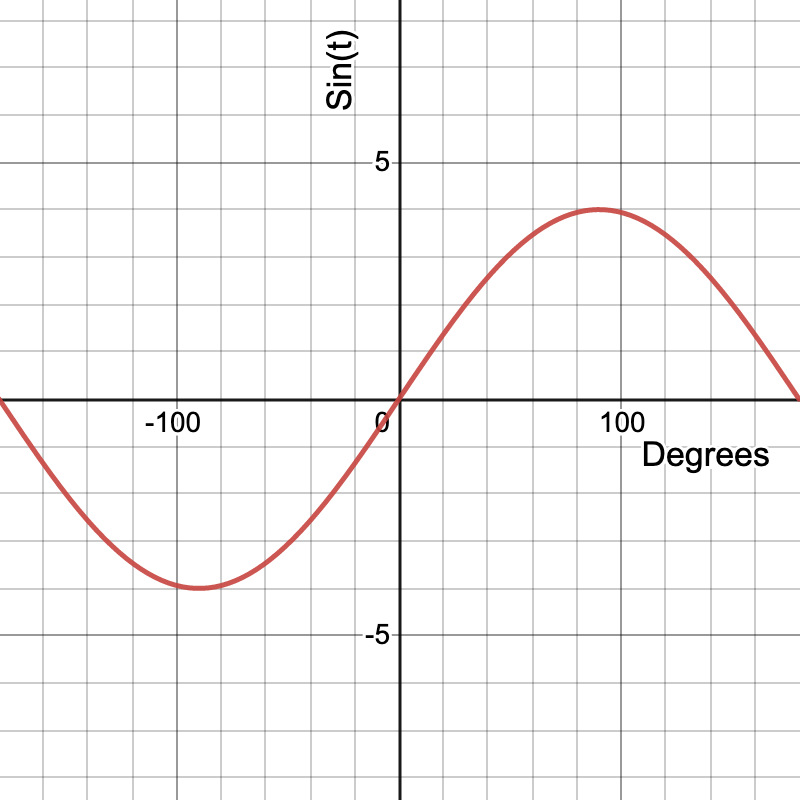
\includegraphics[width=0.40\columnwidth]{sine.png}
   \label{fig:sine}
 }
\hspace{0.2in}
\subfigure[cosine function]{
   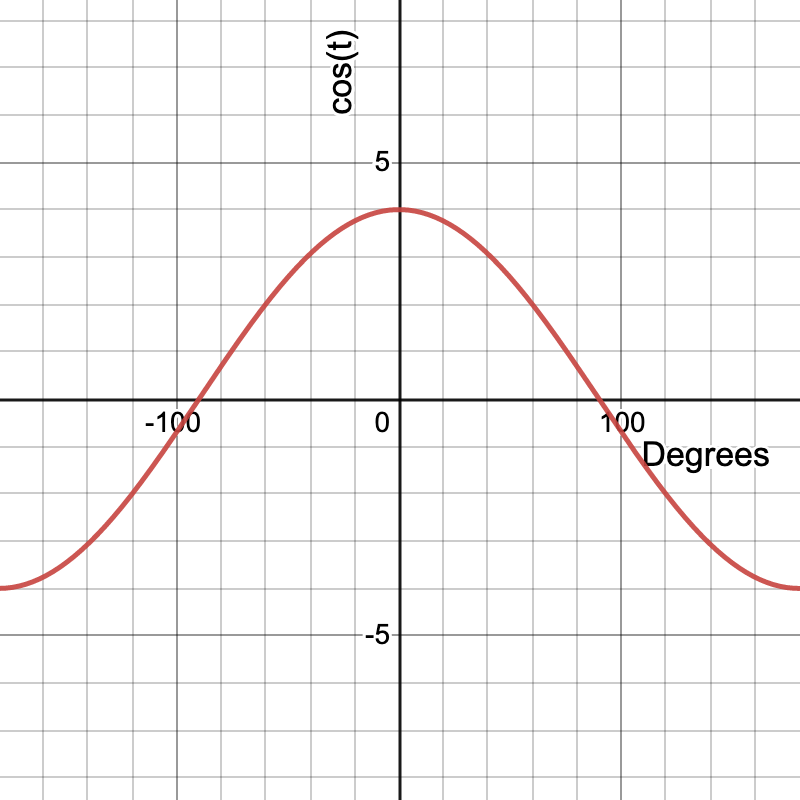
\includegraphics[width=0.40\columnwidth]{cosine.png}
   \label{fig:cosine}
 }
\end{center}
\caption{\small Examples of an odd function (left subfigure) and an even function (right subfigure).  The $\sin{(t)}$ function is odd,  with $\sin{(-t)}=-\sin{(t)}$, while the $\cos{(t)}$ function is even, with $\cos{(-t)}=\cos{(t)}$.}
\label{fig:sinusoids}
\end{figure}

\hspace{.1in}
\subsubsection*{\color{mygreen} Orthogonal functions}

First, a word about orthogonality as you have experienced it before - any vector may be written as a combination of  orthogonal components in the directions of an orthogonal basis,

\[
\vec{v} = v_{x}\hat{x} +v_{y}\hat{y} +v_{z}\hat{z}
\]

Any of these orthogonal vector components may be determined {\it independently} of the others.  Each component is a projection of the vector onto that direction, 

\begin{equation}
\vec{v} = (\vec{v}\cdot \hat{x})\hat{x} +(\vec{v}\cdot \hat{y})\hat{y} + (\vec{v}\cdot \hat{z})\hat{z}
\label{eq:vect_comp}
\end{equation}

Similarly, a function may be approximated by a linear combination of orthogonal basis functions.

\begin{equation}
\begin{aligned}
& f(t) = \sum_{n=0}^{\infty} \, A_{n}\, \phi_{n} \\
& \phi_{n} \hspace{.2in} \longrightarrow \hspace{.2in} \text{orthogonal basis functions} \\
& A_{n}  \hspace{.2in} \longrightarrow \hspace{.2in} \text{constant coefficients} 
\label{eq:series_orth}
\end{aligned}
\end{equation}

The basis functions are orthogonal to insure `finality of coefficients'.   This means it is possible to determine a coefficient in the expansion without knowing the others.  Then for example, more terms of the expansion may be added to the approximation without requiring that earlier terms be `revised'.  The other coefficients remain unchanged.  An orthogonal set of basis functions, $\phi$ satisfy the following {\it orthogonality relation}:

\begin{equation*}
%\begin{rcases}
\int_{I} \phi_{n}(t) \phi_{k}(t) \, dt \hspace{.1in} = \hspace{.2in}
%\end{rcases}
\begin{cases}
 & \hspace{.1in} 0 \hspace{.27in}  k \neq n \\
 & \hspace{.1in} \lambda_{n}  \hspace{.2in}  k=n
\end{cases}
\end{equation*}
where $\lambda_{n}$ is a constant, and the $I$ on the integral means that the integration {\bf must} be over the characteristic interval over which the functions are defined.  

The Kronecker Delta function is often used to make orthogonality conditions more compact.  The definition of the Kronecker Delta is,

\begin{equation*}
%\begin{rcases}
\delta_{ij} = \hspace{.2in}
%\end{rcases}
\begin{cases}
 & \hspace{.1in} 0 \hspace{.27in}  i \neq j \\
 & \hspace{.1in} 1  \hspace{.25in}  i=j
\end{cases}
\end{equation*}

Then,
\tcbset{highlight math style={colframe=myblue,colback=white}}
\begin{empheq}[box=\tcbhighmath]{equation}
\int_{I} \phi_{n}(t) \phi_{k}(t) \, dt \hspace{.2in} = \hspace{.2in} \lambda_{n} \, \delta_{nk}
\label{eq:orthogonality}
\end{empheq}

The orthogonality condition is used to find expressions for the coefficients $A_{n}$ in the expansion.  For example, suppose we want to find the $A_{3}$ coefficient.  Multiply both sides of Eq.~\ref{eq:series_orth} by $\phi_{3}$ and integrate over the characteristic interval $I$:

\begin{eqnarray*}
\int_{I} f(t) \phi_{3}(t) dt  & = &  \sum_{n=0}^{\infty} \, A_{n}\, \int_{I} \phi_{n}(t) \phi_{3}(t) dt \\
 & =  & A_{0} \int_{I} \phi_{0}(t) \phi_{3}(t) dt + A_{1} \int_{I} \phi_{1}(t) \phi_{3}(t) dt+ A_{2} \int_{I} \phi_{2}(t) \phi_{3}(t) dt \\
 & &   \hspace{.2in} + A_{3} \int_{I} \phi_{3}(t) \phi_{3}(t) dt + A_{4} \int_{I} \phi_{4}(t) \phi_{3}(t) dt \ldots \\
& =  & A_{3} \int_{I} \phi_{3}(t) \phi_{3}(t) dt \hspace{.3in} \text{\color{myblue} All other terms are zero} \\
\vspace{.05in}\\
& =  & A_{3} \lambda_{3}
\end{eqnarray*}

Solving for $A_{3}$:
\[
 A_{3} =\frac{1}{\lambda_{3}} \int_{I} f(t) \phi_{3}(t) dt 
\]

Or, in general for coefficient $A_{n}$:
\begin{equation}
 A_{n} =\frac{1}{\lambda_{n}} \int_{I} f(t) \phi_{n}(t) dt 
 \label{eq:coefficient}
\end{equation}

Substitute the result Eq.~\ref{eq:coefficient} into Eq.~\ref{eq:series_orth} to compare with Eq.~\ref{eq:vect_comp},

\begin{eqnarray*}
f(t) & = & \sum_{n=0}^{\infty} \, A_{n}\, \phi_{n} = \sum_{n=0}^{\infty} \, \left[  \frac{1}{\lambda_{n}} \int_{I} f(t) \phi_{n}(t) dt  \right] \, \phi_{n} \\
\vec{v} & = & \sum_{n} (\vec{v}\cdot \hat{n})\hat{n}
\end{eqnarray*}

The basis functions $\phi_{n}$ are analogous to the basis vectors $\hat{n}$.  The vector $\vec{v}$ is projected onto a basis vector direction to give the component in that direction, $v_{n}=\vec{v}\cdot \hat{n}$.  The function $f(t)$ is projected onto a basis function $\phi_{n}$ by taking the inner product $\frac{1}{\lambda_{n}} \int_{I} f(t) \phi_{n}(t) dt$ to give the coefficient for that basis function.


\subsubsection*{\bf \color{mygreen} Sinusoidal orthoganol functions}

Sinusoidal functions (either sines or cosines) and their harmonics provide orthogonal sets of basis functions.  The following set of sine functions is an example of orthogonal basis functions:

\begin{equation*}
\begin{aligned}
& \phi_{1} = \sin{(k_{0}x)} \\
& \phi_{2} = \sin{(2k_{0}x)} \\
& \phi_{3} = \sin{(3k_{0}x)} \\
& \hspace{.5in} \vdots \\
&\phi_{n} = \sin{(nk_{0}x)} \\
\end{aligned}
\end{equation*}
here $k_{0}=\frac{2\pi}{\lambda_{0}}$, where $\lambda_{0}$ is the wavelength of the fundamental sine wave.  

The first harmonic $\phi_{1}$, also called the fundamental, has one oscillation over the characteristic interval $I=\lambda_{0}$.  The second harmonic, $\phi_{2}$, will have two oscillations in the distance $I=\lambda_{0}$, and so on.  The parameter $k$ is called the `wave number', and here $k=nk_{0}$  has $n$ oscillations in the distance $\lambda_{0}$.  If the sinusoidal harmonics were time oscillations rather than position oscillations, they would be written,
\begin{equation*}
\begin{aligned}
& \phi_{1} = \sin{(\omega_{0}t)} \\
& \phi_{2} = \sin{(2\omega_{0}t)} \\
& \phi_{3} = \sin{(3\omega_{0}t)} \\
& \hspace{.5in} \vdots \\
&\phi_{n} = \sin{(n\omega_{0}t)} \\
\end{aligned}
\end{equation*}
where now $\omega_{0}=\frac{2\pi}{\text{T}_{0}}$, where T$_{0}$ is the period of the fundamental sine wave.

The first harmonic $\phi_{1}$, also called the fundamental, has one oscillation over the characteristic time  interval $I=\text{T}_{0}$.  The second harmonic, $\phi_{2}$, will have two oscillations in the time $I=\text{T}_{0}$, and so on.  The parameter $\omega$ is the angular frequency, and here $\omega=n\omega_{0}$  has $n$ oscillations in the time T$_{0}$.

The orthogonality condition for the position dependent sine functions is the following:

\tcbset{highlight math style={colframe=myblue,colback=white}}
\begin{empheq}[box=\tcbhighmath]{equation}
%\begin{rcases}
\int_{0}^{\lambda_{0}} \sin{(nk_{0}x)}\sin{(mk_{0}x)} \, dx \hspace{.1in} = \hspace{.2in}
%\end{rcases}
\begin{cases}
 & \hspace{.1in} 0 \hspace{.27in}  n \neq m \\
 & \hspace{.1in} \frac{\lambda_{0}}{2}  \hspace{.2in}  n=m
\end{cases}
\label{eq:ortho_sine}
\end{empheq}

The integral of Eq.~\ref{eq:ortho_sine} can be explicitly evaluated for both cases ($m=n$ and $m\ne n$ to show the validity of the expression.  When {\color{myred} $\mathbf{n=m}$}, the integral in eq.~\ref{eq:ortho_sine} becomes:
\[
\int_{0}^{\lambda_{0}} \sin^{2}{(nk_{0}x)} \, dx 
\]

Making the substitution $u=nk_{0}x$, then $du=d(nk_{0}x)=nk_{0}dx \rightarrow dx=\frac{1}{nk_{0}}u$.  The limits of integration may need to change as well: checking, $x=0 \rightarrow u= nk_{0}0 = 0$ and $x=\lambda_{0}=\frac{2\pi}{k_{0}} \rightarrow u= nk_{0}\frac{2\pi}{k_{0}} = 2\pi n$ .  Then rewriting the integral,
\[
\frac{1}{nk_{0}} \int_{0}^{2\pi n} \sin^{2}{(u)} \, du
\]

Replace $\sin^{2}{(u)}$ using a trigonometric identity, and integrate,
\begin{eqnarray*}
\frac{1}{nk_{0}} \int_{0}^{2\pi n} \frac{1}{2}\left( 1-\cos{(2u)} \right) \, du & = &
\frac{1}{2nk_{0}} \int_{0}^{2\pi n}  \, du -\frac{1}{4nk_{0}}\int_{0}^{2\pi n} \cos{(2u)} \, d(2u)\\
& = & \frac{1}{2nk_{0}} ( (2 \pi n) - 0 ) -\frac{1}{4nk_{0}} (\sin{(4\pi n)}- \sin{(0)})\\
& = & \frac{\lambda_{0}}{2}
\end{eqnarray*}

On the other hand, when {\color{myred} $\mathbf{n\ne m}$}, the integral in Eq.~\ref{eq:ortho_sine} becomes:

\begin{equation}
\int_{0}^{\lambda_{0}} \sin{(nk_{0}x)}\sin{(mk_{0}x)} \, dx
\label{eq:nnotm} 
\end{equation}

It is convenient to use another trigonometric identity:
\[
\sin{(nk_{0}x)}\sin{(mk_{0}x)} = \frac{1}{2}\left[ \cos{((n-m)k_{0}x)} - \cos{((n+m)k_{0}x)} \right]
\]

Using this identity, Eq.~\ref{eq:nnotm} becomes:
\begin{eqnarray*}
& & \frac{1}{2}\left[ \int_{0}^{\lambda_{0}} \cos{((n-m)k_{0}x)} \, dx - \int_{0}^{\lambda_{0}} \cos{((n+m)k_{0}x)} \, dx \right] \\
& =& \frac{1}{2}\left[ \frac{1}{(n-m)k_{0}} \int_{0}^{2\pi (n-m)} \cos{(u)} \, du - \frac{1}{(n+m)k_{0}} \int_{0}^{2\pi (n+m)} \cos{(u)} \, du \right] \\
& =& \frac{1}{2}\left[ \frac{1}{(n-m)k_{0}} [ \sin{(2\pi (n-m))} - \sin{(0)} ] - \frac{1}{(n+m)k_{0}} [ \sin{(2\pi (n+m))} -\sin{(0)} ] \right] \\
& = & 0
\end{eqnarray*}

So, the orthogonality condition, Eq.~\ref{eq:ortho_sine} is verified.  The harmonics of the cosine function can be shown to be orthogonal functions in the same way.

\subsubsection*{\bf \color{mygreen} Fourier series on a finite repeating interval}

If a function $f(x)$ is defined on an interval, say $-\frac{L}{2}<x<\frac{L}{2}$, and periodic with period $L$ (that is, $f(x+L)=f(x)$.  To expand this function into a set of basis functions, the basis functions must also be periodic with period $L$.

\begin{equation}
f(x) = \frac{a_{0}}{2} + \sum_{n=1}^{\infty} a_{n}\cos{\left(\frac{2\pi nx}{L}\right)} + \sum_{n=1}^{\infty} b_{n}\sin{\left(\frac{2\pi n x}{L}\right)}
\label{eq:fourier}
\end{equation}

Note that if $f(x)$ is an even function, then the sine terms will vanish, since they are odd.  If $f(x)$ is an odd function, the cosine terms will vanish since they are even.  The constant term will vanish as long as the value of $f(x)$ over the interval averages to zero.

The coefficients are the following:
\begin{eqnarray*}
\begin{aligned}
& a_{n}=\frac{2}{L}\int_{-\frac{L}{2}}^{\frac{L}{2}} f(x) \cos{\left( \frac{2\pi n x}{L} \right)} dx \\
& b_{n}=\frac{2}{L}\int_{-\frac{L}{2}}^{\frac{L}{2}} f(x) \sin{\left( \frac{2\pi n x}{L} \right)} dx \\
& \frac{a_{0}}{2}=\frac{1}{L}\int_{-\frac{L}{2}}^{\frac{L}{2}} f(x) dx \\
\end{aligned}
\end{eqnarray*}

The coefficients were found by multiplying both sides of Eq.~\ref{eq:fourier} by the respective orthogonal functions, integrating over the characteristic interval, and then invoking the orthogonality relations.  For example, finding the coefficients in the cosine series requires use of the orthogonality relation for cosines:

\begin{equation*}
%\begin{rcases}
\int_{-\frac{L}{2}}^{\frac{L}{2}} \cos{\left( \frac{2\pi n x}{L} \right)} \cos{\left( \frac{2\pi m x}{L} \right)} dx \hspace{.1in} = \hspace{.2in}
%\end{rcases}
\begin{cases}
 & \hspace{.1in} 0 \hspace{.27in}  k \neq n \\
 & \hspace{.1in} \frac{L}{2}  \hspace{.2in}  k=n
\end{cases}
\label{eq:sinusoidal_orthogonality}
\end{equation*}

\vspace{.1in}
{\color{grey} \hrulefill}\\
{\color{mygreen} Example problem (find the Fourier series representation of a function):}\\

Find a Fourier series that represents the voltage function, $V(x)$, shown in Fig.~\ref{fig:sqpulses}.
\begin{figure}[h]
\centering
\includegraphics*[trim=0cm 0cm 0cm 0cm, clip=true, width=0.7\columnwidth]{sqpulses.png}
\caption{\small Voltage waveform of repeating square pulses.}
\label{fig:sqpulses}
\end{figure}

The general Fourier expansion is as follows,

\begin{equation*}
f(x) = \frac{a_{0}}{2} + \sum_{n=1}^{\infty} a_{n}\cos{\left(\frac{2\pi nx}{L}\right)} + \sum_{n=1}^{\infty} b_{n}\sin{\left(\frac{2\pi n x}{L}\right)}
\end{equation*}

The voltage function is an even function $V(-x)=V(x)$, so the odd series vanishes, all $b_{n}=0$.  The characteristic interval (repeat distance) is $L=a$, so that:

\begin{equation}
V(x) = \frac{a_{0}}{2} + \sum_{n=1}^{\infty} a_{n}\cos{\left(\frac{2\pi nx}{a}\right)}
\label{eq:fscos}
\end{equation}

where,

\[
\frac{a_{0}}{2} = \frac{1}{a}\int_{-\frac{a}{2}}^{\frac{a}{2}} V(x) dx = \frac{1}{a}\int_{-b}^{b} V dx = \frac{2Vb}{a}
\]

The coefficients $a_{n}$ are found by multiplying Eq.~\ref{eq:fscos} by the orthogonal function $\cos{(\frac{2\pi m x}{a})}$ and integrating over the interval:

\begin{eqnarray*}
\int_{-\frac{a}{2}}^{\frac{a}{2}} V(x)\cos{(\frac{2\pi m x}{a})} dx & = & \int_{-\frac{a}{2}}^{\frac{a}{2}} \frac{a_{0}}{2}\cos{(\frac{2\pi m x}{a})}dx + \int_{-\frac{a}{2}}^{\frac{a}{2}}\sum_{n=1}^{\infty} a_{n}\cos{\left(\frac{2\pi nx}{a}\right)}\cos{(\frac{2\pi m x}{a})} dx\\
\int_{-b}^{b} V\cos{(\frac{2\pi m x}{a})} dx & = & \frac{2Vb}{a}\int_{-\frac{a}{2}}^{\frac{a}{2}} \cos{(\frac{2\pi m x}{a})}dx + \sum_{n=1}^{\infty} a_{n}\int_{-\frac{a}{2}}^{\frac{a}{2}}\cos{\left(\frac{2\pi nx}{a}\right)}\cos{(\frac{2\pi m x}{a})} dx\\
\int_{-b}^{b} V\cos{(\frac{2\pi m x}{a})} dx & = & \frac{2Vb}{a}\frac{a}{2\pi m}\int_{-m\pi}^{m\pi} \cos{(u)}du + \sum_{n=1}^{\infty} a_{n}\frac{a}{2}\delta_{nm}\\
\int_{-b}^{b} V\cos{(\frac{2\pi m x}{a})} dx & = & 0 + \frac{a}{2} a_{m}
\end{eqnarray*}

This gives us a solution for the coefficient $a_{m}$:

\begin{equation*}
\begin{aligned}
& a_{m} = \frac{2}{a} \left( \frac{a}{2\pi m} \right) \int_{-\frac{2\pi m b}{a}}^{\frac{2\pi m b}{a}} V\cos{(u)} du \\
& a_{m} = \frac{V}{\pi m}  \left[ \sin{\left(\frac{2\pi m b}{a}\right)} - \sin{\left(-\frac{2\pi m b}{a}\right)} \right]  \\
& a_{m} = \frac{2V}{\pi m} \sin{\left(\frac{2\pi m b}{a}\right)}
\end{aligned}
\end{equation*} 

where $\sin{(-\theta)}=-\sin{(\theta)}$ was used.  Using this result for the coefficients, the specific Fourier series for this potential waveform is the following:

\begin{equation*}
V(x) = \frac{2Vb}{a} + \frac{2V}{\pi}\sum_{n=1}^{\infty} \frac{1}{n}\sin{\left(\frac{2\pi n b}{a}\right)}\cos{\left(\frac{2\pi nx}{a}\right)}
\end{equation*}

{\color{grey} \hrulefill}\\

\subsubsection*{\bf \color{mygreen} Legendre polynomials are orthoganol functions}

Legendre polynomials are an orthogonal set of basis functions.  A Legendre polynomial of of order $l$ is denoted as $P_{l}(\cos{(\theta)})$, or equivalently $P_{l}({x})$ with $x=\cos{(\theta)}$.  A list of the first six Legendre polynomials parameterized in $x$ follows:

\begin{eqnarray*}
P_{0}(x) & = & 1 \\
P_{1}(x) & = & x \\
P_{2}(x) & = & \frac{1}{2}(3x^{2}-1) \\
P_{3}(x) & = & \frac{1}{2}(5x^{3}-3x) \\
P_{4}(x) & = & \frac{1}{8}(35x^{4}-30x^{2}+3) \\
P_{5}(x) & = & \frac{1}{8}(63x^{5}-70x^{3}+15x)
\end{eqnarray*}

The orthogonality condition for the Legendre polynomials is the following,
\begin{equation}
\int_{0}^{\pi} \, P_{l}(\cos{(\theta)})P_{l^{\prime}}(\cos{(\theta)})\sin{(\theta)}d\theta \hspace{.1in} = \hspace{.2in}
\begin{cases}
 & \hspace{.2in} 0 \hspace{.27in}  l \neq l^{\prime} \\
 & \hspace{.1in} \frac{2}{2l+1}  \hspace{.2in}  l=l^{\prime}
\end{cases}
\label{eq:withcos}
\end{equation}

The limits of integration are over the entire interval defined for $\theta$, which in spherical coordinates is $0-\pi$.

Note that
\begin{align}
& d\cos{(\theta)} = -\sin{(\theta)}d\theta \\
& \cos{(0)}=1 \\
& \cos{(\pi)}=-1
\end{align}

So, using these and making the variable substitution $\cos{(\theta)}=x$ in Eq.~\ref{eq:withcos}, the orthogonality condition becomes,

\begin{eqnarray*}
-\int_{0}^{\pi} \, P_{l}(\cos{(\theta)})P_{l^{\prime}}(\cos{(\theta)})d\cos{(\theta)} & = &  
\int_{\pi}^{0} \, P_{l}(\cos{(\theta)})P_{l^{\prime}}(\cos{(\theta)})d\cos{(\theta)} \\
& = & \int_{-1}^{1} \, P_{l}(x)P_{l^{\prime}}(x) dx \\
& = & \frac{2}{2l+1} \delta_{ll^{\prime}}
\end{eqnarray*}

Summarizing the orthogonality condition for Legendre polynomials:

\tcbset{highlight math style={colframe=myblue,colback=white}}
\begin{empheq}[box=\tcbhighmath]{equation}
\int_{-1}^{1} \, P_{l}(x)P_{l^{\prime}}(x) dx = \int_{0}^{\pi} \, P_{l}(\cos{(\theta)})P_{l^{\prime}}(\cos{(\theta)})\sin{(\theta)}d\theta = \frac{2}{2l+1} \delta_{ll^{\prime}}
\label{eq:legendre_orthogonality}
 \end{empheq}

Notice that Legendre polynomials with $l$ even are even functions, while polynomials with $l$ odd are odd functions, or stating this another way,
\[
P_{l}(-x)=(-1)^{l} \, P_{l}(x)
\]

\begin{figure}[h]
\centering
\includegraphics*[trim=0cm 0cm 0cm 0cm, clip=true, width=0.5\columnwidth]{polynomials.png}
\caption{\small Legendre polynomials $P_{0}(x)-P_{3}(x)$.}
\label{fig:polynomials}
\end{figure}

Figure \ref{fig:polynomials} shows a plot of the first four Legendre polynomials, $P_{0}(x)-P_{3}(x)$.  It can be seen in the figure that $P_{0}(x)$ and $P_{2}(x)$ are even functions, while $P_{1}(x)$ and $P_{3}(x)$.  This is discernible from the analytic expressions; $P_{l}(x)$ with $l$ odd has only odd powers of $x$, and $P_{l}(x)$ with $l$ even has only even powers of $x$.

\begin{figure}[h]
\begin{center}
\subfigure[even and odd]{
   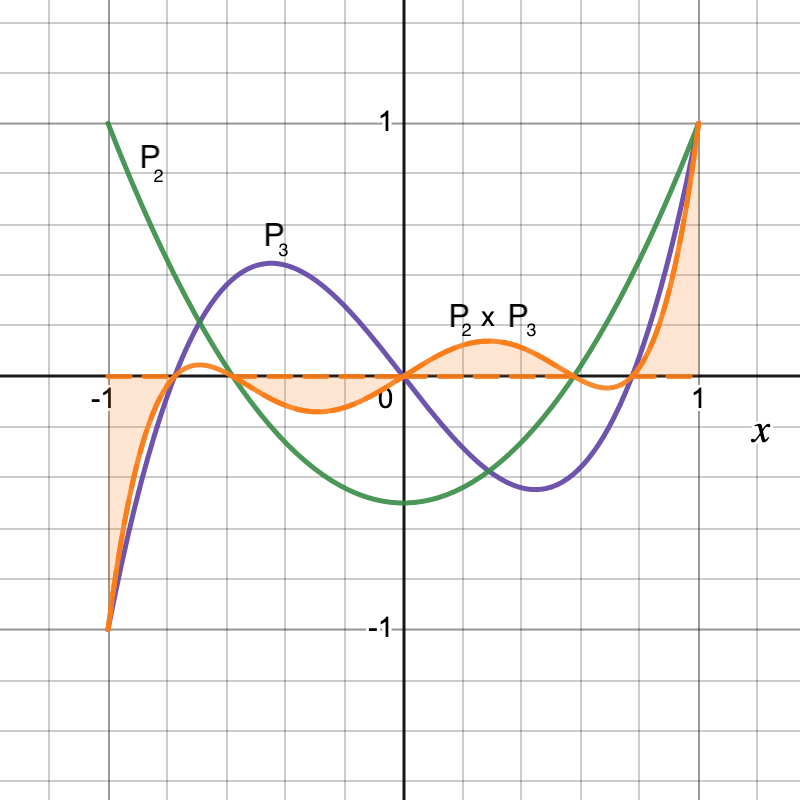
\includegraphics[width=0.42\columnwidth]{P2_P3.png}
   \label{fig:p2p3}
 }
\hspace{0.2in}
\subfigure[odd and odd]{
   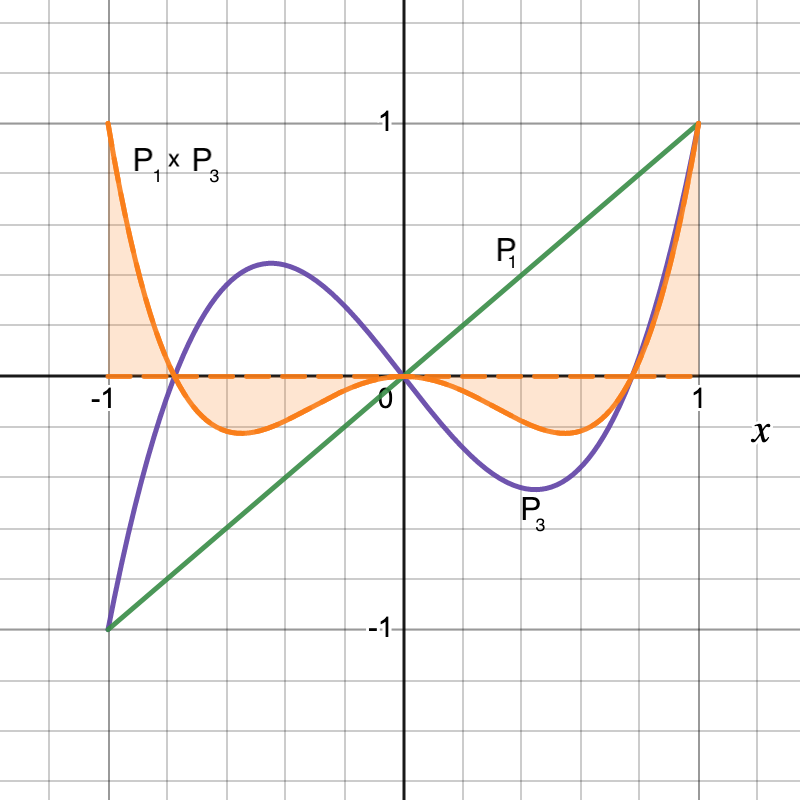
\includegraphics[width=0.42\columnwidth]{P1_P3.png}
   \label{fig:p1p3}
 }
\end{center}
\caption{\small Examples of two Legendre polynomials and their product over the interval.  The area under the curve of the product of the two functions is shaded.  \textcolor{blue} {Left:} The $P_{2}(x)$ (green curve) and $P_{3}(x)$ (purple curve) polynomials, and their product $P_{2}(x) \times P_{3}(x)$ (orange curve).  The area under the curve would be added up to get the integrated  product of the functions (in this case, an even and odd function).  The net area is clearly zero.  \textcolor{blue} {Right:} The $P_{1}(x)$ (green curve) and $P_{3}(x)$ (purple curve) polynomials, and their product $P_{1}(x) \times P_{3}(x)$ (orange curve).  The area under the curve would be added up to get the integrated  product of the functions (in this case, two odd functions).  The net area is still zero, but it is more difficult to tell, better to do the integration to be sure.}
\label{fig:polyproducts}
\end{figure}


\end{flushleft}
\end{document}